\documentclass[conference]{IEEEtran}
\usepackage{amsmath,amssymb}
\usepackage{graphicx}
\usepackage{booktabs}
\usepackage{array}
\usepackage{url}
\usepackage{xurl}
\usepackage[colorlinks=true,linkcolor=black,citecolor=black,urlcolor=blue]{hyperref}
\usepackage{balance}

\graphicspath{{figures/}}

\newcommand{\mamba}{Mamba}

\begin{document}

\title{Efficient Sequence Modeling: From S4D to \mamba{}-3\\
\large An Experimental Study of Five Sequence Architectures in Pure PyTorch}

\author{\IEEEauthorblockN{Vaibhav Mahore}
\IEEEauthorblockA{\textit{Department of Mathematics and Computing}\\
\textit{Indian Institute of Science, Bangalore, India}\\
mvaibhav@iisc.ac.in}}

\maketitle

\begin{abstract}
Quadratic attention cost limits Transformer-based sequence models at long
context, motivating a family of recurrent alternatives culminating in
selective state space models (SSMs) such as \mamba{}. This paper presents an
experimental study in which five sequence backbones: a causal Transformer,
S4D, \mamba{}-1, \mamba{}-2 (chunked State Space Duality), and
\mamba{}-3 (complex-valued transitions with exponential-trapezoidal
discretization) are implemented from first principles in pure PyTorch,
share one training skeleton, and are verified by equivalence tests that check
independent computational forms of the same mathematics against each other.
All architectures are evaluated on three tasks probing different
capabilities (parity state tracking, selective copying, IMDb sentiment
classification) and benchmarked for latency, peak memory, and throughput at
sequence lengths from 1K to 32K on a single 6\,GB consumer GPU. The study
reproduces capability claims of the \mamba{}-3 literature at small scale:
complex-valued transitions solve a cumulative-parity tracking task at
98.3\% token accuracy where real-transition SSMs and the Transformer remain
at chance, and LTI S4D collapses to 6\% token accuracy on selective copying
while selective SSMs reach 67\%. Efficiency measurements show the quadratic
training cost of attention in wall-clock terms (30\,ms per step at 1K tokens
versus 186\,s at 32K), that the FFT-convolution form of S4D is the most
wall-clock-efficient implementation in this codebase across the measured
range, and that educational sequential scans are $O(T)$ in operations but
10--100$\times$ slower in wall-clock, quantifying the gap between asymptotic
complexity and hardware behavior. All results are produced by committed
scripts from committed result files, and all scope restrictions (S4D rather
than full S4, no \mamba{}-3 MIMO path, no fused kernels) are stated.
\end{abstract}

\begin{IEEEkeywords}
state space models, S4D, Mamba, selective scan, state space duality, length
generalization, sequence modeling, efficiency benchmarking
\end{IEEEkeywords}

\section{Introduction}
Modeling dependencies over long sequences is a central requirement in
language, audio, and time-series applications. The dominant architecture,
the Transformer \cite{vaswani2017attention}, computes pairwise interactions
between all positions: self-attention costs $O(T^2)$ in compute for sequence
length $T$. Memory-efficient attention kernels reduce activation memory but
not the asymptotic compute, and the cost of long-context training and
inference remains substantial.

State space models (SSMs) offer an alternative: a linear recurrence over a
fixed-size hidden state with $O(T)$ total operations and constant per-token
state at inference \cite{gu2022efficiently,gu2021lssl}. The S4 family
introduced structured, HiPPO-initialized transition matrices that endow the
recurrence with long-range memory \cite{gu2020hippo}, computed either as a
recurrence or, for linear time-invariant (LTI) systems, as a convolution.
\mamba{} \cite{gu2023mamba} made the transition parameters input-dependent
(selectivity), \mamba{}-2 \cite{dao2024transformers} restricted the
transition to a scalar per head so that the recurrence can be evaluated as
chunked matrix products (State Space Duality, SSD), and \mamba{}-3
\cite{lahoti2026mamba3} restored expressivity needed for state tracking
through complex-valued transitions and a more accurate discretization rule.

This paper documents an experimental study built around five from-scratch
implementations of these architectures. The goals are threefold: (1) verify
that the mathematical claims of each architecture hold when the recurrence is
written out and tested, (2) measure which capabilities each architecture
actually exhibits on small controlled tasks, and (3) quantify the gap between
asymptotic complexity and wall-clock performance on consumer hardware. The
contributions are:

\begin{itemize}
\item Five sequence backbones (Transformer, S4D, \mamba{}-1, \mamba{}-2 with
a chunked SSD scan, \mamba{}-3 with complex transitions and
exponential-trapezoidal discretization) implemented in pure PyTorch behind a
single shared interface, with no dependency on fused SSM kernels.
\item Equivalence tests that verify independent computational forms of the
same mathematics (FFT-convolution versus recurrent stepping; chunked SSD
versus a sequential reference; \mamba{}-3 versus the \mamba{}-1/2 update in
its limiting configuration), which caught four real implementation bugs
during development.
\item A three-task capability study (cumulative-parity state tracking,
selective copying, IMDb sentiment) at matched training budgets, reproducing
the capability claims of the \mamba{}-3 and \mamba{} literature at small
scale.
\item A sequence-length efficiency sweep (1K--32K) measuring training-step
latency, peak memory, throughput, and decode cost on a 6\,GB RTX 4050
Laptop GPU, with measured hardware limits recorded rather than omitted.
\end{itemize}

Scope: the S4 implementation is the diagonal S4D restriction
\cite{gu2022s4d}, not full Normal-Plus-Low-Rank S4; \mamba{}-3 covers the
recurrence but not its MIMO formulation or chunked dual; scans are
educational, not kernel-fused. These restrictions are reflected throughout.

\section{Background: State Space Models}

\subsection{Continuous-Time Formulation}
A (diagonal) SSM maps a 1-D input $u(t)$ to an output $y(t)$ through a hidden
state $x(t)\in\mathbb{C}^{N}$ governed by
\begin{equation}
\dot{x}(t) = A\,x(t) + B\,u(t), \qquad y(t) = \mathrm{Re}\!\left(\sum_{n} C_n x_n(t)\right) + D\,u(t),
\label{eq:cont}
\end{equation}
where $A=\mathrm{diag}(A_1,\dots,A_N)$ holds the per-slot transition
parameters, $B$ injects the input, $C$ reads the state, and $D$ is a skip
connection. The real part of $A_n$ controls decay and the imaginary part
controls rotation frequency; stability requires
$\mathrm{Re}(A_n)<0$.

\subsection{Discretization}
Because tokens are discrete, the system is integrated with step size
$\Delta$. Under zero-order-hold (ZOH) discretization with diagonal $A$,
\begin{equation}
\bar{A}_n = e^{\Delta A_n}, \qquad
\bar{B}_n = \Delta B_n \,\phi(\Delta A_n), \quad \phi(z) = \frac{e^{z}-1}{z}.
\label{eq:zoh}
\end{equation}
The factor $\phi(z)$ tends to $1$ as $z\to 0$; evaluating it naively produces
a $0/0$ condition, so the implementation uses a Taylor fallback
$\phi(z)\approx 1+z/2+z^2/6$ for $|z|<10^{-4}$ and the closed form elsewhere.
The discretized system is the linear recurrence
\begin{equation}
x_t = \bar{A}\,x_{t-1} + \bar{B}\,u_t .
\label{eq:disc}
\end{equation}

\subsection{Convolution and Recurrence: Two Forms of One System}
Unrolling \eqref{eq:disc} for an LTI system yields $y = K * u$ with kernel
\begin{equation}
K_k = \sum_{n=0}^{N-1} C_n \bar{B}_n \bar{A}_n^{\,k}, \qquad
\bar{A}_n^{\,k} = e^{k\Delta A_n}.
\label{eq:kernel}
\end{equation}
Because $\bar{A}_n^k$ is an exponential in $k$ (a Vandermonde structure), the
kernel is computed without iterating powers, and the training-time output is
a causal FFT convolution computed in $O(T\log T)$. At inference, the same
system advances with $O(1)$ work per token using
\eqref{eq:disc} directly. The two forms are mathematically identical, a
property our test suite exploits (Section~\ref{sec:impl}).

\section{Architectures}
All five backbones share one skeleton: token embedding, a stack of
pre-norm residual blocks, a final normalization, masked mean pooling, and a
linear classification head. Table~\ref{tab:arch} summarizes the mixer inside
each block.

\begin{table}[t]
\centering
\caption{The five implemented mixers. ``E-Euler'' denotes the
exponential-Euler rule ($\bar A = e^{\Delta A}$, input scaled by $\Delta B$)
later formalized by the \mamba{}-3 paper.}
\label{tab:arch}
\small
\begin{tabular}{@{}p{0.135\columnwidth}p{0.22\columnwidth}p{0.24\columnwidth}p{0.22\columnwidth}@{}}
\toprule
Model & Transition $A$ & Training form & Decode \\
\midrule
Transformer & -- & causal SDPA attention & full-prefix recompute \\
S4D & complex diagonal, HiPPO-style init & FFT convolution, $O(T\log T)$ & $O(1)$-state complex step \\
\mamba{}-1 & real negative diagonal, input-dependent $\Delta,B,C$ & selective scan (loop) & incremental step, $O(1)$ state \\
\mamba{}-2 & scalar-per-head $\times I$ & chunked SSD matmuls & sequential scan \\
\mamba{}-3 & complex diagonal, input-dependent & selective scan & sequential scan \\
\bottomrule
\end{tabular}
\end{table}

\subsection{S4D}
The S4D restriction \cite{gu2022s4d} keeps a complex diagonal transition
$A_n=-\exp(a_n) + i\pi n$ (S4D-Lin initialization), a per-channel step size
$\Delta$ mapped through a softplus into $[10^{-3},10^{-1}]$, and complex
input/output vectors $B,C$ initialized at scale $1/\sqrt{N}$. Training uses
the FFT convolution of \eqref{eq:kernel} with a chunked kernel computation
(chunks of 1024 positions); decode uses a complex state of shape
$(B,D,N)$ updated once per token. The block applies a SiLU gate on a second
linear branch, so although the recurrence is LTI the block is not.

\subsection{\mamba{}-1: Selectivity}
\mamba{} \cite{gu2023mamba} makes $\Delta_t$, $B_t$, and $C_t$ functions of
the input through a linear projection, breaking the LTI assumption and with
it the convolution form: the system becomes time-varying and training
requires a scan. With $\alpha_t = e^{\Delta_t A}\in(0,1)$,
\begin{equation}
x_t = \alpha_t\, x_{t-1} + \Delta_t B_t\, u_t .
\label{eq:selective}
\end{equation}
The block is: input projection to two branches, a causal short convolution
(kernel 4), SiLU activation, the selective scan, a SiLU gate, and an output
projection under a pre-norm residual. The $\Delta$ projection bias is
initialized log-uniformly in $[10^{-3},10^{-1}]$ so that different state
slots operate at different timescales. Decode maintains both the SSM state
and the convolution history, one token at a time.

\subsection{\mamba{}-2: State Space Duality}
\mamba{}-2 \cite{dao2024transformers} restricts the transition to a scalar
per head, $A = a_h\,\mathbb{I}$. The unrolled recurrence then factors into a
lower-triangular decayed sum that resembles attention:
\begin{equation}
Y = \bigl(L \odot (C B^{\top})\bigr) X + \text{carry-in}, \qquad
L_{ts} = \prod_{r=s+1}^{t}\alpha_r = e^{cs_t - cs_s},
\label{eq:ssd}
\end{equation}
where $cs$ is the cumulative sum of $\log\alpha$ and $L$ is masked to the
lower triangle. The sequence is processed in chunks of size $C$: within a
chunk, outputs are computed as decayed, masked matmuls; across chunks, a
state $S\in\mathbb{R}^{N\times P}$ is carried with
$S \leftarrow \alpha^{\mathrm{tot}} S + \sum_t \alpha^{\mathrm{suf}}_t\,
B_t\otimes x_t$. This reduces the sequential loop length by a factor of $C$
and turns the inner computation into tensor-core matmuls, which is the
practical reason \mamba{}-2 exists. Our implementation processes chunks in
groups to bound transient memory.

\subsection{\mamba{}-3: Complex Transitions and a Better Rule}
\mamba{}-3 \cite{lahoti2026mamba3} addresses a capability gap: transitions
with real non-negative eigenvalues can only decay state; they cannot rotate
it, which formally limits state tracking. The implemented recurrence adds
two of the three paper contributions. First, exponential-trapezoidal
discretization approximates the state-input integral with a data-dependent
combination of both endpoints,
\begin{equation}
x_t = \alpha_t x_{t-1} + \underbrace{(1-\lambda_t)\,\Delta_t \alpha_t\, B_{t-1} u_{t-1}}_{\beta_t} + \underbrace{\lambda_t \Delta_t}_{\gamma_t} B_t u_t,
\label{eq:trap}
\end{equation}
with $\lambda_t=\sigma(\cdot)\in(0,1)$; setting $\lambda_t=1$ recovers the
exponential-Euler rule of \mamba{}-1/2, and the rule is second-order
accurate. Second, the transition becomes complex, $A=-\exp(a)+i\theta$: the
magnitude $|\alpha_t| = e^{-\Delta_t \exp(a)}<1$ guarantees stability
independent of phase, while the phase $\Delta_t\theta$ rotates the state by
an input-dependent angle. The paper's MIMO formulation is described but not
implemented here.

\subsection{Transformer Baseline}
The baseline is a pre-norm causal Transformer using
\texttt{scaled\_dot\_product\_attention} (memory-efficient kernels) with
sinusoidal positions. No KV cache is implemented; decode cost is therefore
reported as honest full-prefix recomputation.

\section{Implementation and Verification}
\label{sec:impl}
The package (2{,}900 lines of Python, no SSM-kernel dependencies) exposes all
backbones behind one registry. Correctness is enforced by equivalence tests
that compare independent implementations of the same mathematics:
the S4D FFT-convolution path against its recurrent step path; the
\mamba{}-2 chunked SSD against a sequential reference scan (chunk sizes 32
and 64, including a padded sequence); \mamba{}-3 against the
\mamba{}-1/2 recurrence at $\lambda_t=1$, $\theta=0$; and \mamba{}-1's
incremental decode against its parallel forward. Agreement is at
$10^{-3}$ absolute tolerance, appropriate for fp32 reassociation. Four
development bugs were caught by these tests (a conjugation-convention
mismatch in S4D, a kernel-chunk concatenation along the wrong axis, a
triangular-mask construction that silently masked nothing, and a conv-state
slice on the wrong axis), supporting the practice of testing independent
derivations. The suite contains 16 tests covering the equivalence checks,
masking, determinism, and dataset contracts.

\section{Experimental Setup}
Three tasks probe different capabilities; all models train under identical
protocols per task (shared data, optimizer, schedule, and seeds; one seed per
configuration).

\textbf{Parity (state tracking).} The target at position $t$ is the XOR of
inputs $1..t$, $L=128$, 20 epochs; the task requires input-dependent rotation
of state.

\textbf{Selective copying.} Marker--value pairs are embedded in a noise
stream; a separator then requests the $k$ remembered values in order. Train
$L=64$ (3--5 pairs), test $L=128$ (5--10 pairs), 12 epochs. Only $k$ values
must be retained (constant in $L$) while noise must be gated out.

\textbf{IMDb sentiment.} Standard binary classification, 12.5k training
subset (fixed seed), maximum length 512, 3 epochs, $d_{\text{model}}=128$,
4 blocks. Sequential-loop models (\mamba{}-1/3) are excluded from IMDb on
wall-clock grounds (Section~VI-D); the selective-SSM family is represented
by \mamba{}-2, which shares their recurrence.

\textbf{Efficiency sweep.} Training-step latency (forward, backward, update;
CUDA events, 5 repeats), peak memory, throughput, and decode cost at
$T\in\{1\mathrm{K},\dots,32\mathrm{K}\}$, batch 8, $d_{\text{model}}=256$,
2 blocks, fp32, on an RTX 4050 Laptop GPU (6\,GB, Windows/WDDM).

\section{Results}

\subsection{Parity: Complex Transitions Enable State Tracking}
Table~\ref{tab:parity} and Fig.~\ref{fig:parity} show the study's headline
capability result. \mamba{}-3 reaches 98.3\% token accuracy (42\% of test
sequences fully correct) while \mamba{}-1, \mamba{}-2, S4D, and the
Transformer remain at 50.6--56.3\% token accuracy with zero fully-correct
sequences. The mechanism is the rotation argument of
\cite{lahoti2026mamba3}: parity requires $x_t = R(\pi u_t)\,x_{t-1}$, a
rotation by an input-dependent angle. Real non-negative transitions cannot
rotate; S4D is complex but LTI, so its rotation angle cannot depend on the
input; only \mamba{}-3's input-dependent complex transition provides both
stability ($|\alpha_t|<1$) and input-dependent phase. The experiment
reproduces the paper's motivating capability claim at small scale.

\begin{table}[t]
\centering
\caption{Cumulative-parity tracking at $L=128$ (20 epochs, matched budgets).}
\label{tab:parity}
\small
\begin{tabular}{@{}lrrr@{}}
\toprule
Model & Params & Token acc. & Seq. success \\
\midrule
Transformer & 100{,}354 & 0.533 & 0.000 \\
S4D & 33{,}794 & 0.507 & 0.000 \\
\mamba{}-1 & 78{,}210 & 0.559 & 0.000 \\
\mamba{}-2 & 68{,}786 & 0.563 & 0.000 \\
\mamba{}-3 & 69{,}562 & \textbf{0.983} & \textbf{0.420} \\
\bottomrule
\end{tabular}
\end{table}

\begin{figure}[t]
\centering
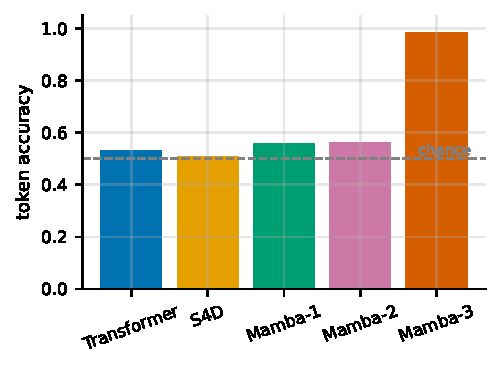
\includegraphics[width=\columnwidth]{parity.pdf}
\caption{Cumulative-parity tracking. Only the complex-transition model
(\mamba{}-3) exceeds the chance line; real-transition SSMs cannot represent
the required input-dependent rotation.}
\label{fig:parity}
\end{figure}

\subsection{Selective Copying: Selectivity Separates Gated from LTI Models}
On selective copying (Fig.~\ref{fig:selcopy}), the selective SSMs lead:
\mamba{}-2 0.670 and \mamba{}-1 0.649 token accuracy (18.3\% and 14.9\%
full-sequence success at test length 128), against Transformer 0.205 and
S4D 0.064. The result illustrates selectivity as designed in
\cite{gu2023mamba}: the task rewards gating noise out of state, which LTI
kernels cannot express. \mamba{}-3 underperforms its real-transition
siblings here (0.215 token accuracy); at this small budget its rotational
dynamics appear to trade recall sharpness for state-tracking power, and we
report this as measured rather than tuning it away.

\begin{figure}[t]
\centering
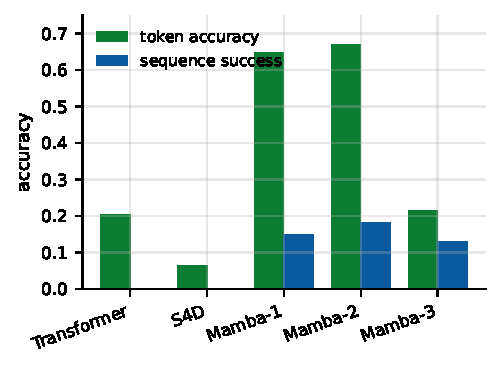
\includegraphics[width=\columnwidth]{selcopy.pdf}
\caption{Selective copying, train $L=64$, test $L=128$. Selective SSMs
retain the $k$ marker--value pairs and gate out noise; LTI S4D cannot and
collapses.}
\label{fig:selcopy}
\end{figure}

\subsection{IMDb Sentiment}
At matched budget on real text (Table~\ref{tab:imdb},
Fig.~\ref{fig:imdb}), \mamba{}-2 attains the best accuracy (0.836) and AUC
(0.917), S4D follows (0.827/0.907), and the Transformer trails
(0.813/0.894). These are single-seed results on a half-data protocol and
should be read as directional evidence, not as a leaderboard.

\begin{table}[t]
\centering
\caption{IMDb sentiment (12.5k train subset, $L\le 512$, 3 epochs).}
\label{tab:imdb}
\small
\begin{tabular}{@{}lrrr@{}}
\toprule
Model & Params & Accuracy & AUC \\
\midrule
Transformer & 3{,}353{,}602 & 0.813 & 0.894 \\
S4D & 2{,}677{,}762 & 0.827 & 0.907 \\
\mamba{}-2 & 3{,}034{,}786 & \textbf{0.836} & \textbf{0.917} \\
\bottomrule
\end{tabular}
\end{table}

\begin{figure}[t]
\centering
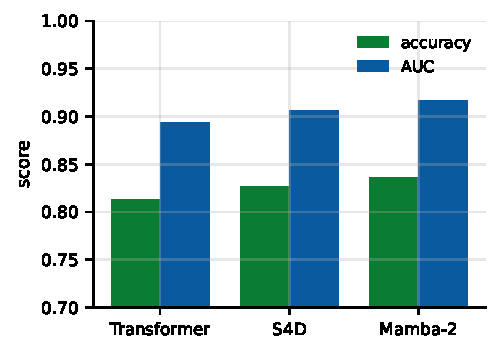
\includegraphics[width=\columnwidth]{imdb.pdf}
\caption{IMDb sentiment at matched budget.}
\label{fig:imdb}
\end{figure}

\subsection{Efficiency: Theory Versus Wall Clock}
Fig.~\ref{fig:eff} and Table~\ref{tab:eff} summarize the sweep. Three
observations, all measured on the same hardware and protocol:

\begin{figure*}[t]
\centering
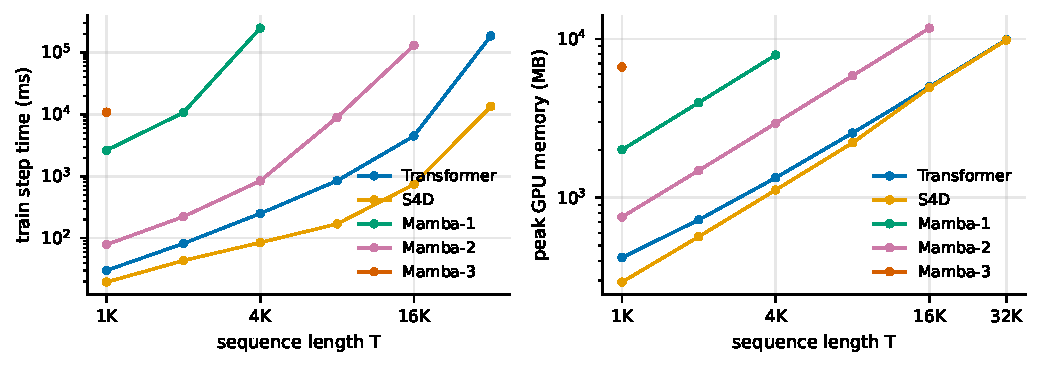
\includegraphics[width=\textwidth]{efficiency.pdf}
\caption{Training-step latency (left) and peak GPU memory (right) versus
sequence length on an RTX 4050 Laptop (6\,GB), batch 8, fp32, CUDA-event
timed over 5 repeats. The Transformer's $O(T^2)$ compute dominates
wall-clock despite memory-efficient attention kernels; S4D's FFT-convolution
form is the most wall-clock-efficient implementation across the measured
range; sequential-scan models are capped by launch overhead and, past 6\,GB,
by shared-memory spill (Mamba-1/3 measured only to their limits; Mamba-2
exceeds memory at 32K).}
\label{fig:eff}
\end{figure*}

\begin{table}[t]
\centering
\caption{Efficiency summary (train step, batch 8; fp32). Dashes: not
measured (loop cost); OOM: measured memory limit.}
\label{tab:eff}
\small
\begin{tabular}{@{}lrr@{}}
\toprule
Model & $T{=}1$K & $T{=}32$K \\
\midrule
Transformer & 30 ms / 419 MB & 186{,}025 ms / 9{,}879 MB \\
S4D (FFT) & 20 ms / 294 MB & 13{,}456 ms / 9{,}820 MB \\
\mamba{}-2 (chunked) & 79 ms / 754 MB & OOM \\
\mamba{}-1 (loop) & 2{,}632 ms / 2{,}000 MB & -- (capped at 4K) \\
\bottomrule
\end{tabular}
\end{table}

\textbf{(a) The quadratic bill is real.} The Transformer's step time grows
from 30\,ms at $T{=}1$K to 186\,s at $T{=}32$K, roughly three orders of
magnitude for a $32\times$ length increase, with the last interval
amplified by WDDM shared-memory spill past the 6\,GB buffer. Attention
kernels improved the constant, not the asymptotics.

\textbf{(b) FFT convolution is hard to beat in wall clock.} S4D is the
fastest implementation at every measured length (13.5\,s per step at 32K),
consistent with a single well-optimized FFT pair per layer versus scans or
matmul chains.

\textbf{(c) $O(T)$ operations can still lose.} The educational sequential
scans perform $O(T)$ work but are 10--100$\times$ slower than vectorized
forms at equal length (2.6\,s versus 30\,ms at $T{=}1$K for \mamba{}-1
versus the Transformer). Each of the $T\times$ layers steps launches small
kernels and extends a $T$-node autograd graph. This is precisely why fused
selective-scan kernels and the chunked SSD matmul form exist, and it is the
study's central complexity-versus-hardware lesson: asymptotics describe how
work grows, packaging determines how fast it runs.

\section{Discussion}
The tasks form a coherent capability picture. Parity shows that the
transition parameterization (complex, input-dependent phase) is a
first-order architectural capability, not an implementation detail;
selective copying shows the LTI family failing for a mechanistic reason;
IMDb shows modest, real differences on natural language, with the SSD-family
model competitive end to end. The efficiency sweep separates these
capability questions from the deployment question, where the S4D
convolution form and, at scale, kernel-fused implementations dominate.

\section{Limitations}
(1) The implementations are educational: python-loop scans are 10--100$\times$
slower in wall-clock than fused kernels, and no comparison against the
official \mamba{} kernels (Linux-only) was run on this machine. (2) Full S4
(NPLR parameterization with Woodbury-corrected Cauchy kernels) is not
implemented; S4D retains the ideas this study needs. (3) \mamba{}-3's MIMO
formulation and chunked dual are not implemented; its recurrence is.
(4) Task results use a single seed; IMDb uses a half-data subset and 512-token
truncation. (5) The efficiency sweep is fp32; bf16 autocast would change
absolute numbers. (6) \mamba{}-1/3 sequential training exceeds the 6\,GB
buffer at $T\ge 2$K, so their long-length training cost is reported as a
measured limit, not extrapolated.

\section{Conclusion}
Five sequence architectures were implemented from first principles behind
one interface, verified by equivalence tests that caught real bugs, and
evaluated across three capability tasks and a 1K--32K efficiency sweep. The
study reproduces, at small scale and with committed evidence, the central
capability claims of the modern SSM literature: input-dependent complex
transitions restore state tracking (98.3\% on parity where all
real-transition baselines remain at chance), input-dependent gating solves
noise-laden retention tasks that defeat LTI models (67\% versus 6\% on
selective copying), and the SSD matmul form is competitive on natural
language. The efficiency measurements ground the asymptotic story in
hardware reality: quadratic attention is visibly quadratic, FFT convolution
is extremely strong in wall clock, and $O(T)$ recursion is only as fast as
its packaging. All code, configs, committed result files, and regeneration
scripts are available in the accompanying repository.\footnote{\url{https://github.com/vaibhav3000/s4-to-mamba}}

\begin{thebibliography}{9}

\bibitem{vaswani2017attention}
A.~Vaswani, N.~Shazeer, N.~Parmar, J.~Uszkoreit, L.~Jones, A.~N. Gomez,
{\L}.~Kaiser, and I.~Polosukhin, ``Attention is all you need,'' in
\emph{Advances in Neural Information Processing Systems (NeurIPS)}, 2017,
arXiv:1706.03762.

\bibitem{gu2020hippo}
A.~Gu, T.~Dao, S.~Ermon, A.~Rudra, and C.~R{\'e}, ``HiPPO: Recurrent memory
with optimal polynomial projections,'' in \emph{Proc. Int. Conf. on Machine
Learning (ICML)}, 2020, arXiv:2008.07669.

\bibitem{gu2021lssl}
A.~Gu, I.~Johnson, K.~Goel, K.~Saab, T.~Dao, A.~Rudra, and C.~R{\'e},
``Combining recurrent, convolutional, and continuous-time models with linear
state space layers,'' in \emph{Advances in Neural Information Processing
Systems (NeurIPS)}, 2021, arXiv:2110.13985.

\bibitem{gu2022efficiently}
A.~Gu, K.~Goel, and C.~R{\'e}, ``Efficiently modeling long sequences with
structured state spaces,'' in \emph{Int. Conf. on Learning Representations
(ICLR)}, 2022, arXiv:2111.00396.

\bibitem{gu2022s4d}
A.~Gu, A.~Gupta, K.~Goel, and C.~R{\'e}, ``On the parameterization and
initialization of diagonal state space models,'' in \emph{Advances in Neural
Information Processing Systems (NeurIPS)}, 2022, arXiv:2206.11893.

\bibitem{gu2023mamba}
A.~Gu and T.~Dao, ``\mamba{}: Linear-time sequence modeling with selective
state spaces,'' 2023, arXiv:2312.00752.

\bibitem{dao2024transformers}
T.~Dao and A.~Gu, ``Transformers are SSMs: Generalized models and efficient
algorithms through structured state space duality,'' in \emph{Proc. Int.
Conf. on Machine Learning (ICML)}, 2024, arXiv:2405.21060.

\bibitem{lahoti2026mamba3}
A.~Lahoti, K.~Y. Li, B.~Chen, C.~Wang, A.~Bick, J.~Z. Kolter, T.~Dao, and
A.~Gu, ``\mamba{}-3: Improved sequence modeling using state space
principles,'' 2026, arXiv:2603.15569.

\end{thebibliography}

\end{document}
